\documentclass[12pt]{article}
\setlength{\oddsidemargin}{0in}
\setlength{\evensidemargin}{0in}
\setlength{\textwidth}{6.5in}
\setlength{\parindent}{0in}
\setlength{\parskip}{\baselineskip}
\usepackage{amsmath,amsfonts,amssymb}
\usepackage{graphicx}
\usepackage[]{algorithmicx}
\usepackage{enumitem}
\usepackage{fancyvrb}

\usepackage{fancyhdr}
\pagestyle{fancy}
\setlength{\headsep}{36pt}

\usepackage{hyperref}
\graphicspath{{F:/Users/sasha/Documents/Summer 2020/Algo/hw 2a}}

\hypersetup{
    colorlinks=true,
    linkcolor=blue,
    filecolor=magenta,      
    urlcolor=blue,
}

\newcommand{\makenonemptybox}[2]{%
%\par\nobreak\vspace{\ht\strutbox}\noindent
\item[]
\fbox{% added -2\fboxrule to specified width to avoid overfull hboxes
% and removed the -2\fboxsep from height specification (image not updated)
% because in MWE 2cm is should be height of contents excluding sep and frame
\parbox[c][#1][t]{\dimexpr\linewidth-2\fboxsep-2\fboxrule}{
  \hrule width \hsize height 0pt
  #2
 }%
}%
\par\vspace{\ht\strutbox}
}
\makeatother

\begin{document}
\lhead{{\bf CSCI 3104, Algorithms \\ Homework 2A (45 points)} }
\rhead{Name: \fbox{% Place your name here and delete the next time
\phantom{This is a really long name}} 
\\ ID: \fbox{ % Place your ID here and delete the next time
\phantom{This is a student ID}} 
\\ {\bf Escobedo \& Jahagirdar\\ Summer 2020, CU-Boulder}}
\renewcommand{\headrulewidth}{0.5pt}

\phantom{Test}

\begin{small}
\textit{Advice 1}:\ For every problem in this class, you must justify your answer:\ show how you arrived at it and why it is correct. If there are assumptions you need to make along the way, state those clearly.
%\vspace{-3mm} 

\textit{Advice 2}:\ Verbal reasoning is typically insufficient for full credit. Instead, write a logical argument, in the style of a mathematical proof.\\
%\vspace{-3mm} 

\textbf{Instructions for submitting your solution}:
\vspace{-5mm} 

\begin{itemize}
	\item The solutions \textbf{should be typed}, we cannot accept hand-written solutions. Here's a short intro to \href{http://ece.uprm.edu/~caceros/latex/introduction.pdf}{\textbf{Latex}.}
	 \item In this homework we denote the asymptomatic \textit{Big-O} notation by $\mathcal{O}$ and \textit{Small-O} notation is represented as $o$. 
	\item We recommend using online Latex editor \href{https://www.overleaf.com/}{\textbf{Overleaf}}. Download the \textbf{.tex} file from Canvas and upload it on overleaf to edit.
	%todo add link of gradescope
	\item You should submit your work through \href{https://www.gradescope.com}{\textbf{Gradescope}}  only.
	\item If you don't have an account on it, sign up for one using your CU email. You should have gotten an email to sign up. If your name based CU email doesn't work, try the identikey@colorado.edu version. 
	\item Gradescope will only accept \textbf{.pdf} files (except for code files that should be submitted separately on Canvas if a problem set has them) and \textbf{try to fit your work in the box provided}. 
	\item You cannot submit a pdf which has less pages than what we provided you as Gradescope won't allow it.
   
\end{itemize}
\vspace{-4mm} 
\end{small}

\hrulefill
\pagebreak

\subsection*{Piazza threads for hints and further discussion}
\begin{center}
    \begin{tabular}{|c|}
    \hline
    Piazza Threads \\ [0.5ex] 
    \hline \hline 
    \href{https://piazza.com/class/ka2roz7rb9m3j4?cid=29}{Question 1}\\
    \href{https://piazza.com/class/ka2roz7rb9m3j4?cid=30}{Question 2}\\
    \href{https://piazza.com/class/ka2roz7rb9m3j4?cid=31}{Question 3}\\
    \href{https://piazza.com/class/ka2roz7rb9m3j4?cid=32}{Question 4}\\
    \href{https://piazza.com/class/ka2roz7rb9m3j4?cid=33}{Question 5}\\
    
    \hline
    \end{tabular}
\end{center}

\textbf{Recommended reading}: Divide \& Conquer; Recurrence Relations: Ch. 2 →  2.3; Ch. 4 →  4.1, 4.2, 4.3, 4.4, 4.5. The three methods for solving recurrences from \textbf{4.3} - \textbf{4.5} is important. 

\pagebreak

\begin{enumerate}

	\item{
	 \itshape (5 $\times$ 4 = 20 pts) Solve the following recurrence relations. For each case, show your work.
	}
	
	\begin{enumerate}[label=(\alph*)]
	 
	\item{
	 \itshape $T(n) = 3T(n-1) + 1$ if $n>1$ and $T(1) = \Theta(1)$ 
	 }
	\makenonemptybox{6.5in}{
	$T(n) = 3T(n-1) + 1$\\
	$= 3(3T(n-2)+1)+1 = 9T(n-2)+3+1$\\
	$=3(9T(n-3)+2+1)+1=27T(n-3)+6+3+1$\\
	.\\
	.\\
	.\\
	$=2^{n-1}T(1)+3^{n-2}+...+3^2+1$\\
	\\
	$\sum_{i=0}^{n}3^i$\\
	\\
	$=\Theta(3^n)$
	}
	
	\pagebreak
	\item
	{
	 \itshape $T(n) = 2T(\frac{n}{3}) + \Theta(n)$ if $n>1$ and $T(1) = \Theta(1)$ 
	 }
	\makenonemptybox{6.5in}{
	$T(n) = 2T(\frac{n}{3}) + \Theta(n)$\\
	Using Master Method\\
	$a= 2$, $b=3$, $c=1$\\
	\\
	We use the case 3 of the Masters Theorem. 3rd case states $\Theta(n^c)$ if $a<b^c$\\
	\\
	Plugging in the respective values we get:\\
	$a<b^c \leftrightarrow \log_b a< \log_b b^c=c$\\
	\\
	$T(n) = n^c \sum_{k=0}^{\log_b n-1}(\frac{a}{b^c})^k+n^{\log_b a}$\\
	\\
	$= n^c\cdot \Theta(1)+n^{\log_b a}$\\
	$=\Theta(n)$
	}
	
	\pagebreak
	
	\item
	{
	 \itshape $T(n) = 3T(\frac{n}{2}) + \Theta(n)$ if $n>1$ and $T(1) = \Theta(1)$
	 }
	\makenonemptybox{6.5in}{
	$T(n) = 3T(\frac{n}{2}) + \Theta(n)$ is best solved using the masters method.\\
	$a = 3$, $b= 2$, $c=1$\\
	\\
	plugging in our values to the third case of the masters theorem $(a > b^c)$we see that the inqualities hold true.\\
	$3 > 2^1$\\
	\\
	Therefore by the master's theorem it states $T(n)= n^c \cdot(\frac{a^{\log_b n}}{n^c})+n^{\log_b a}$\\
	$= n^c \cdot (n^{\log_2 3})+n^{\log_2 3}$\\
	$=\Theta(n^{\log_2 3})$
	}
	
	\pagebreak
	 
	 
	 \item
	 {
	 \itshape $T(n) = 4T(\frac{n}{2}) + \Theta(n^2)$ if $n>1$ and $T(1) = \Theta(1)$ 
	 }
	\makenonemptybox{6.5in}{
	$T(n) = 4T(\frac{n}{2}) + \Theta(n^2)$ is best solved using the masters theorem.\\
	\\
	$a=4$, $b=2$, $c= 2$\\
	Plugging in our values into the second case of the masters method $(a=b^c)$ we can se that it holds true.\\
	$4=2^2$\\
	\\
	Therefore by the masters thereom, the second case states:\\
	$T(n)= \sum_{k=0}^{\log_b n-1}(\frac{a}{b^c})^k+n^{\log_b a}$\\
	\\
	$= n^c \cdot \Theta(\log_b n)+n^{\log_b a}$\\
	$=\Theta(n^{2}\log_2 n)$
	}
	
	\pagebreak
	 \end{enumerate}
	 
	 \item{
	 \itshape (5 pts) Can master's theorem be applied to solve the following recurrence \\
	 $T(n) = 8T(\frac{n}{2}) + n^3 \log(n)$. If $n>1$ and $T(1) = \Theta(1)$}\\
	  {Prove that the above recurrence cannot be solved using Master's theorem by showing that none of the three conditions required to apply the theorem are satisfied by the recurrence.}
	 \makenonemptybox{6in}{
	 Yes we can apply Master's Theorem to the recurrence  however it cannot be used to solve it because none of the three cases are satisfied by the recurrence.\\ $T(n) = 8T(\frac{n}{2}) + n^3 \log(n)$\\\\
	 $a=8$, $b=2$, $f(n)=n^3\log n$, $n^{\log_b a} = n^{\log_2 8}= \mathcal{O}(n^3)$\\
	 \\
	 Case 01:\\
	 $states f(n) = \mathcal{O}(n^{\log_b a + c}) $ where c represents some constant.\\
	 $n^3 \cdot \log n \neq n^3$
	 We can see that this expression does not hold and therefore does not satisfy the first case of masters theorem.\\
	 
	 Case 02, 03:\\
	$f(n)> n^{\log_b a}=n^3$, although this is a true statement, f(n) is not polynomially larger.
	$\frac{f(n)}{n^{\log_b a}}= \frac{n^3 \log n}{n^3}= \log n$. Thi ratio is asymptotically less than $n^k$ for any positive constant k. Therefore this recurrrence falls into the gap of Case 02 and Case 03.
	}
	\pagebreak
	
	\item{
	\itshape  (5 $\times$ 2 = 10 pts) Consider the following functions. For each of them, determine how many times is ‘hi’ printed in terms of the input n (i.e in Asymptotic Notation of n). You should first write down a recurrence and then
solve it using the \textbf{recursion tree method}. That means you should write down the
first few levels of the recursion tree, specify the pattern, and then solve.
	}
	 
	\begin{enumerate}[label=(\alph*)]
	    \item
	    \begin{Verbatim}[numbers=left,xleftmargin=15mm, numbersep=10pt]
def fun(n) {
    if (n > 1) {
        print( ‘hi’ ‘hi’ ‘hi’ )
        fun(n/3)
        fun(n/3)
    }
}
            \end{Verbatim}
        \makenonemptybox{5in}{
        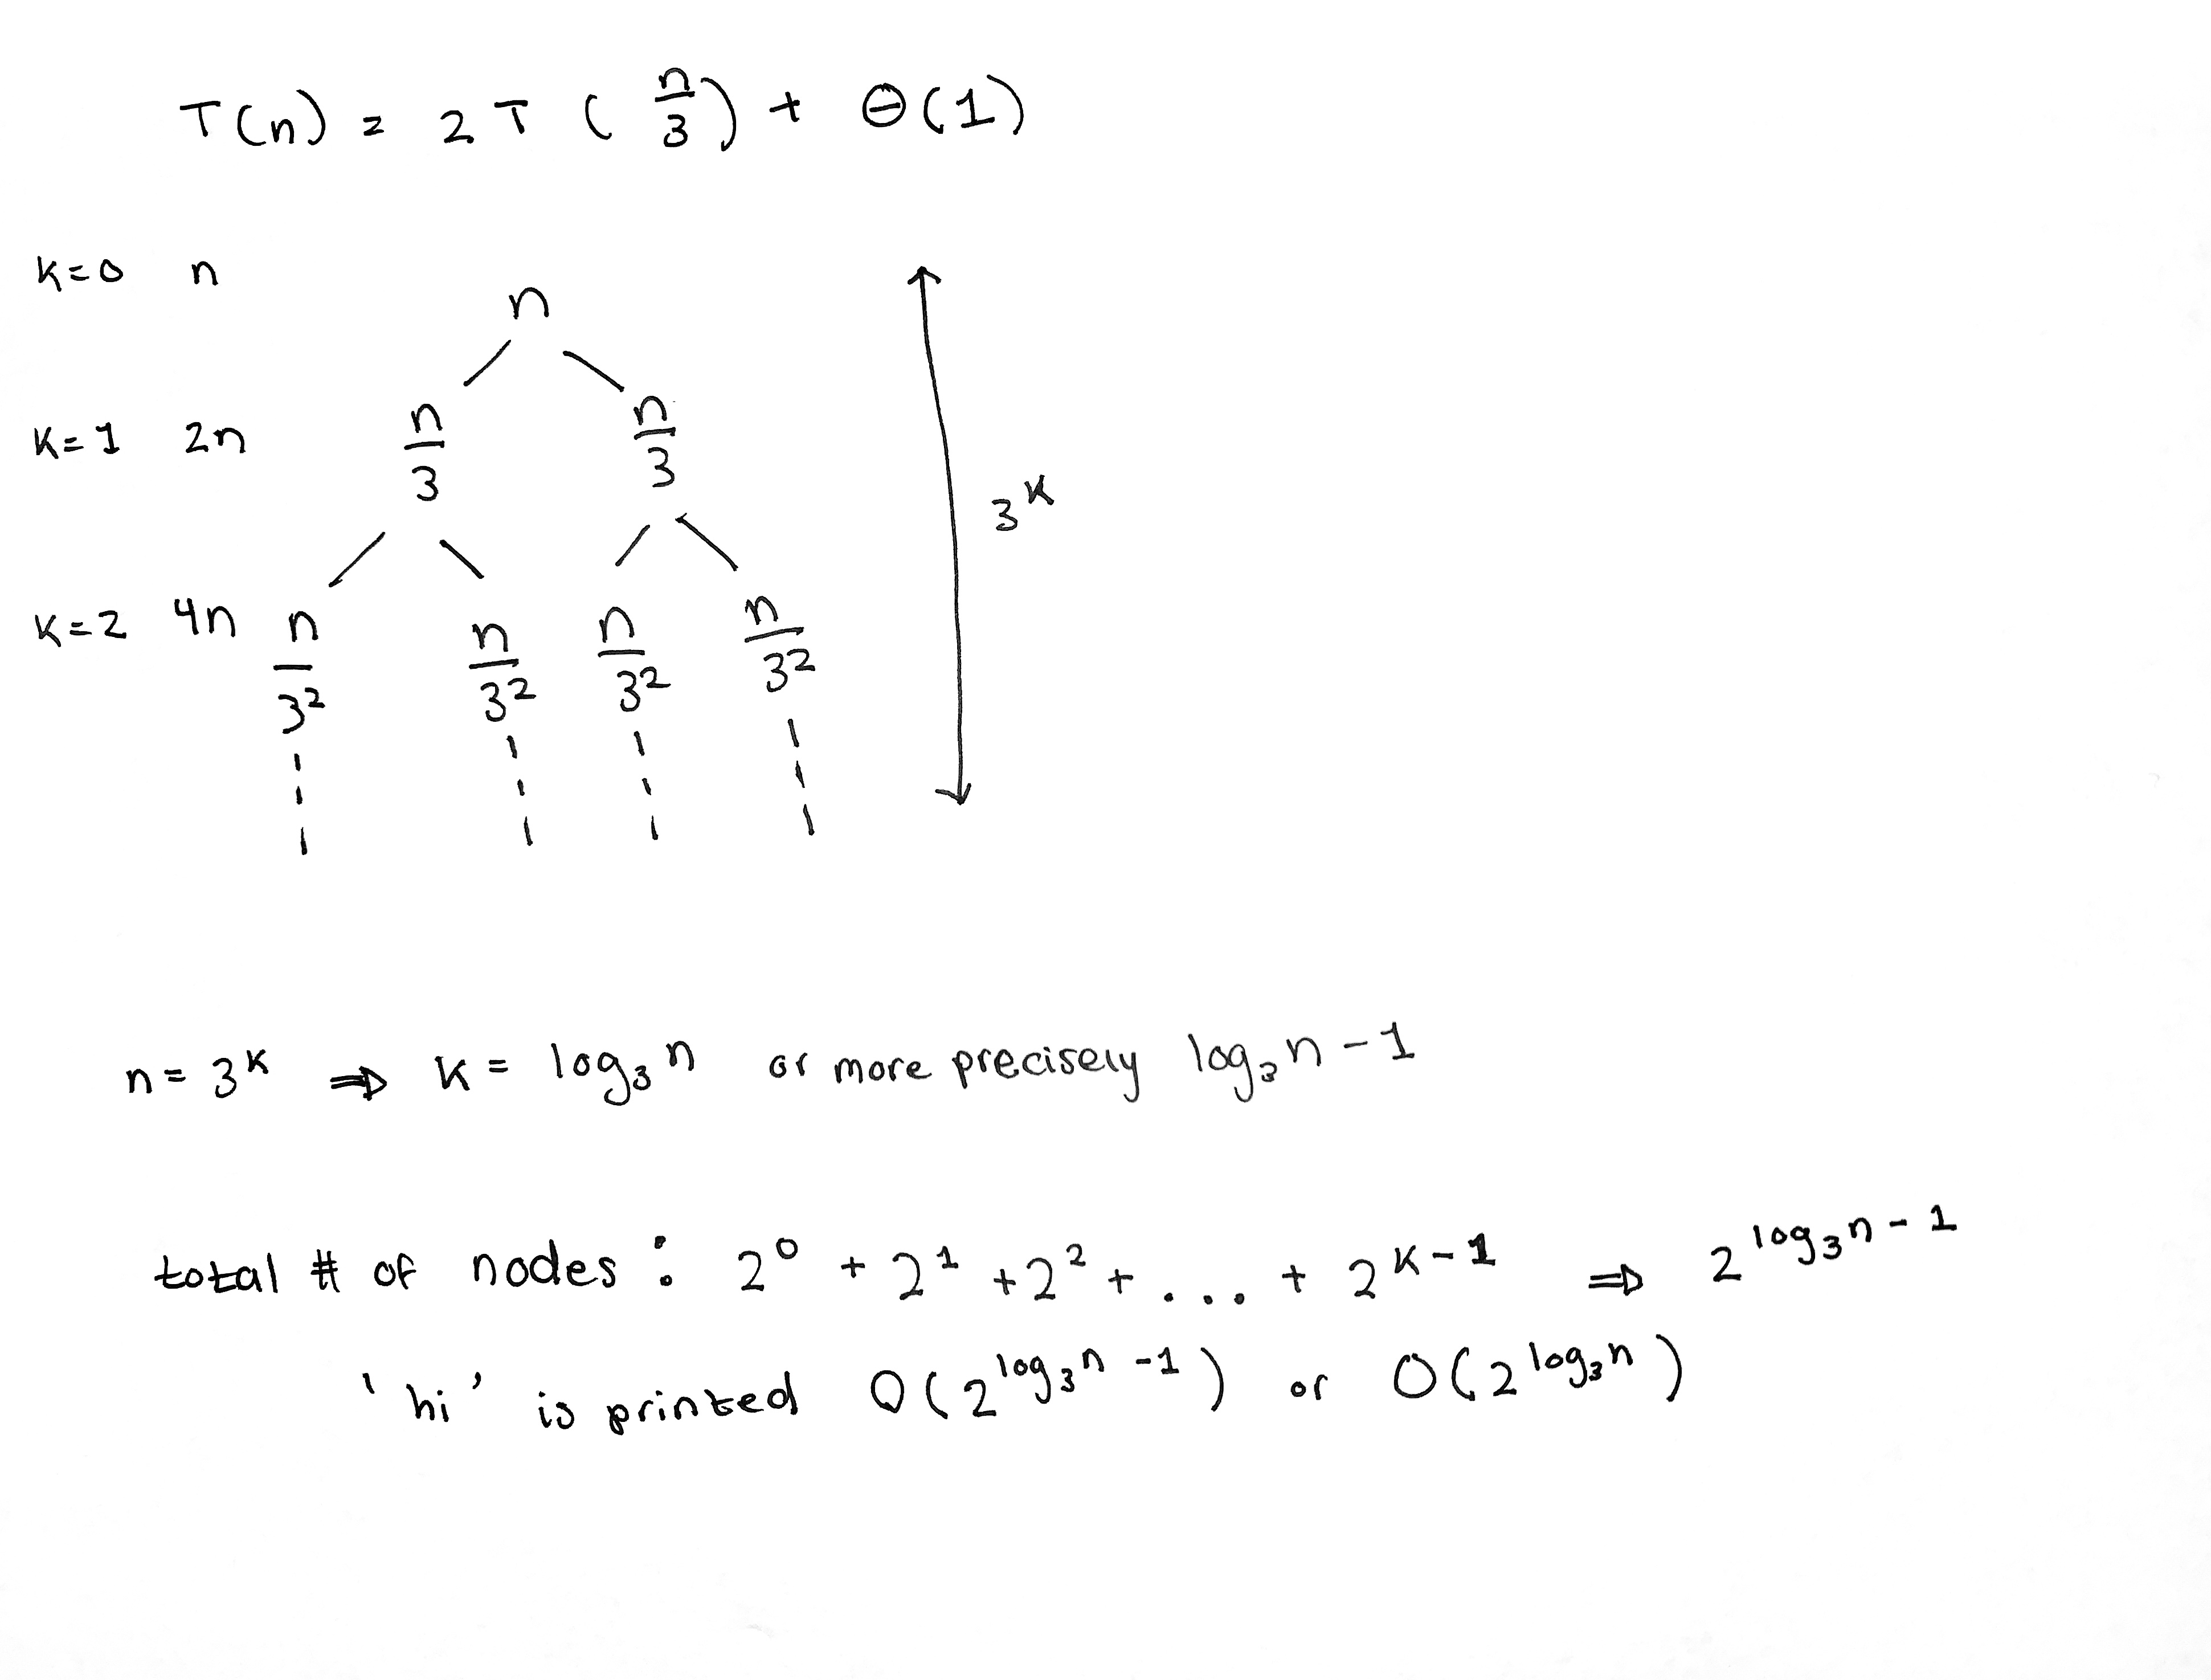
\includegraphics[scale=0.1]{solution3a.jpg}\\
        \\
        $T(n)=\mathcal{O}(2^{\log_3 n})$
	    }
	    \pagebreak
	    \item 
	    \begin{Verbatim}[numbers=left,xleftmargin=15mm, numbersep=10pt]
def fun(n) {
    if (n > 1) {
        for i=1 to n {
            print( ‘hi’ ‘hi’ )
        }
        fun(n/3)
        fun(n/3)
    }
}	        
	    \end{Verbatim}
	    \makenonemptybox{5.5in}{
	            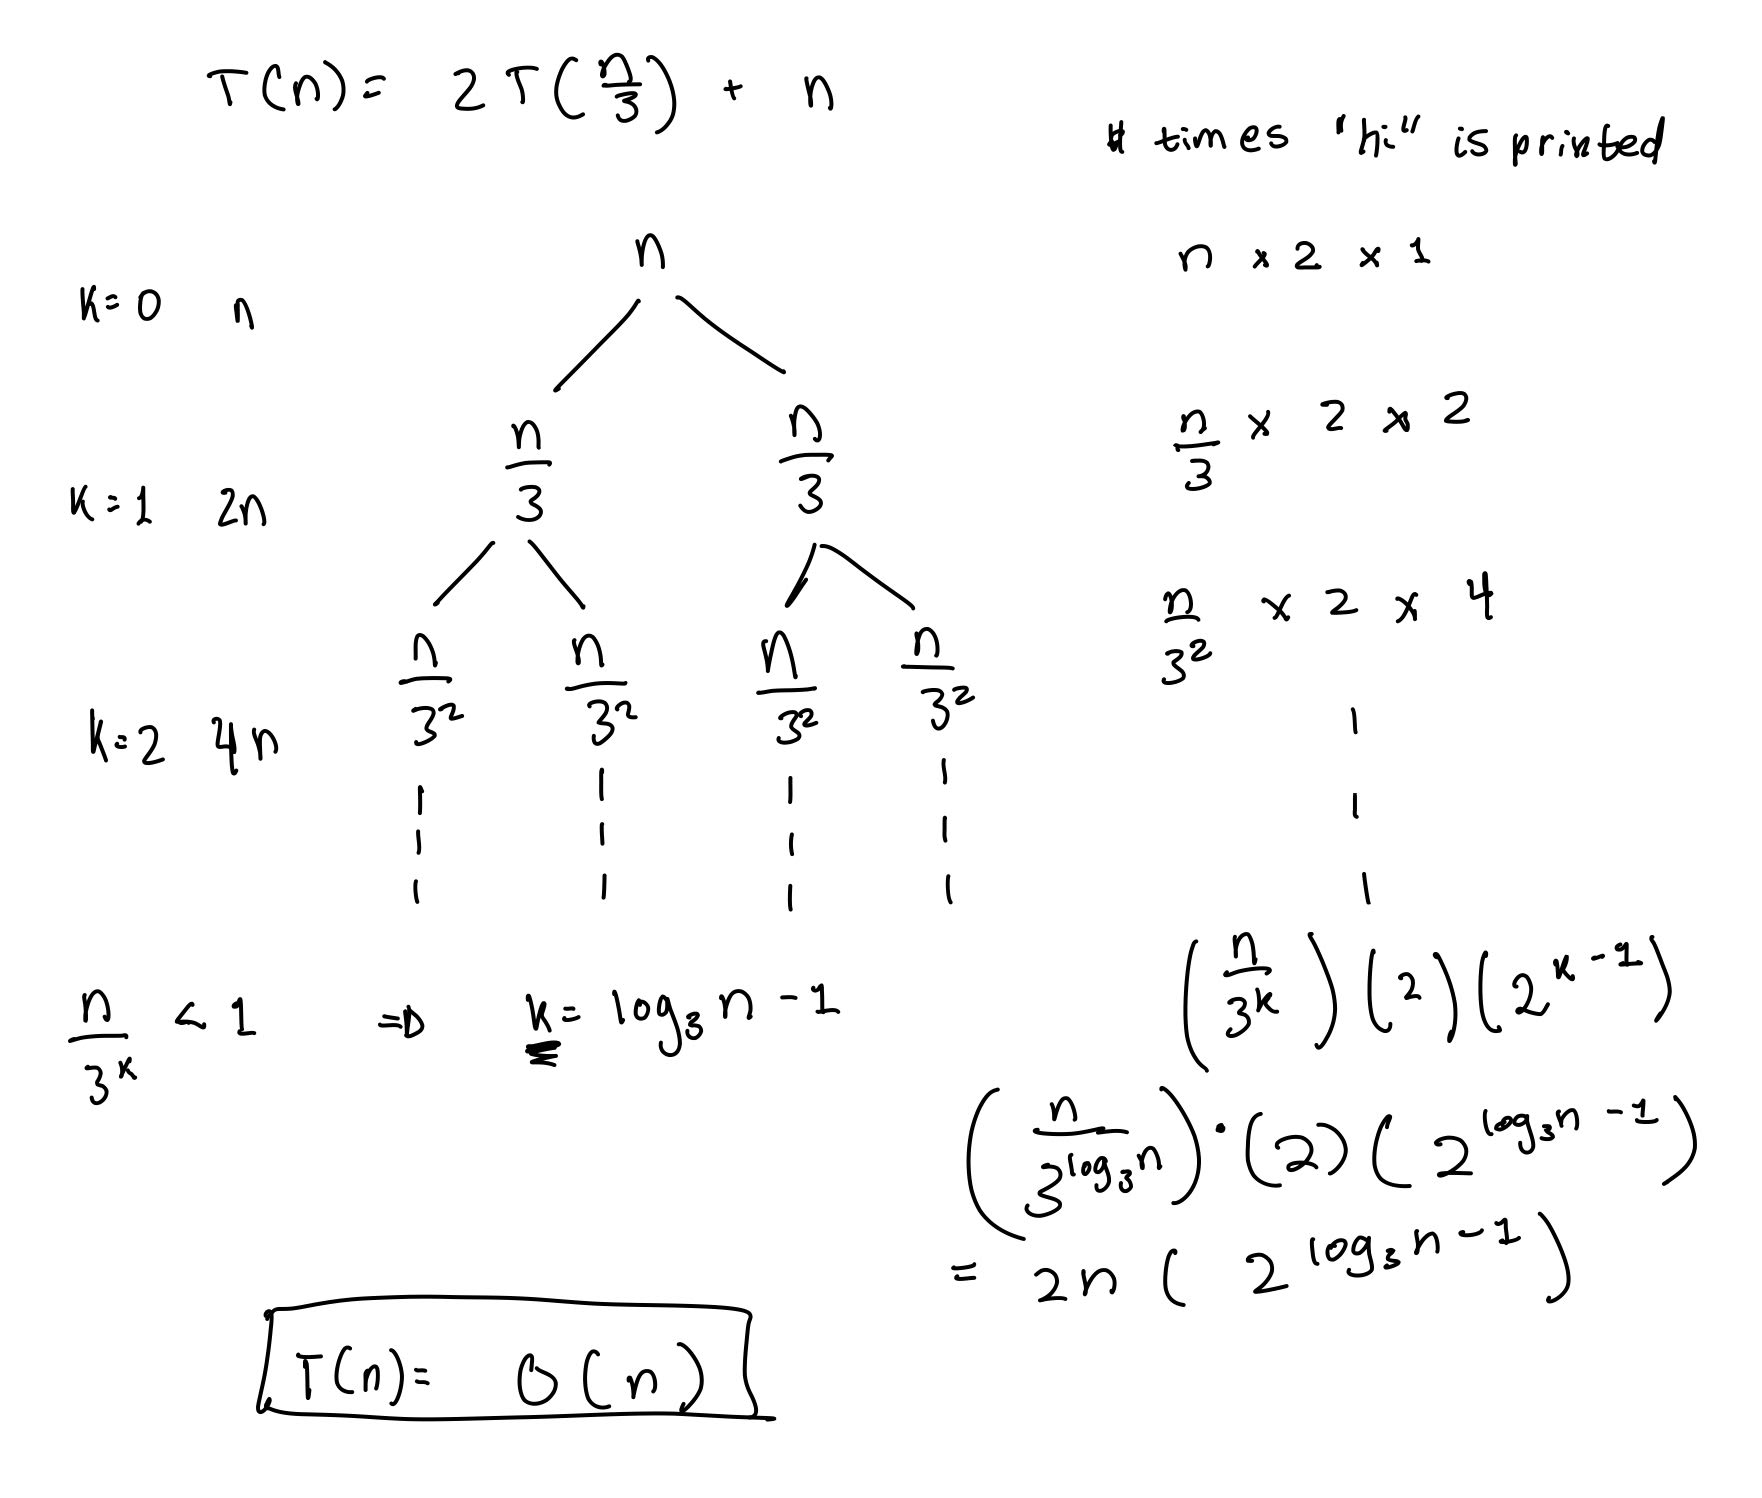
\includegraphics[scale=0.2]{solution3b.jpg}\\
	            $T(n)=\mathcal{O}(n)$
	    }
	    
	\end{enumerate}
	\pagebreak
	\item{
	\itshape  (5 pts)
	Let $T(n) = 3T(\frac{n}{3}) + n$, where $T(n)$ is constant when $n \leq 3$. Using unrolling, determine tight asymptotic bounds for $T(n)$.  That is, find a function $g(n)$ such that $T(n) \in \Theta(g(n)$). Clearly show all your work
	}
	\makenonemptybox{6.5in}{
	    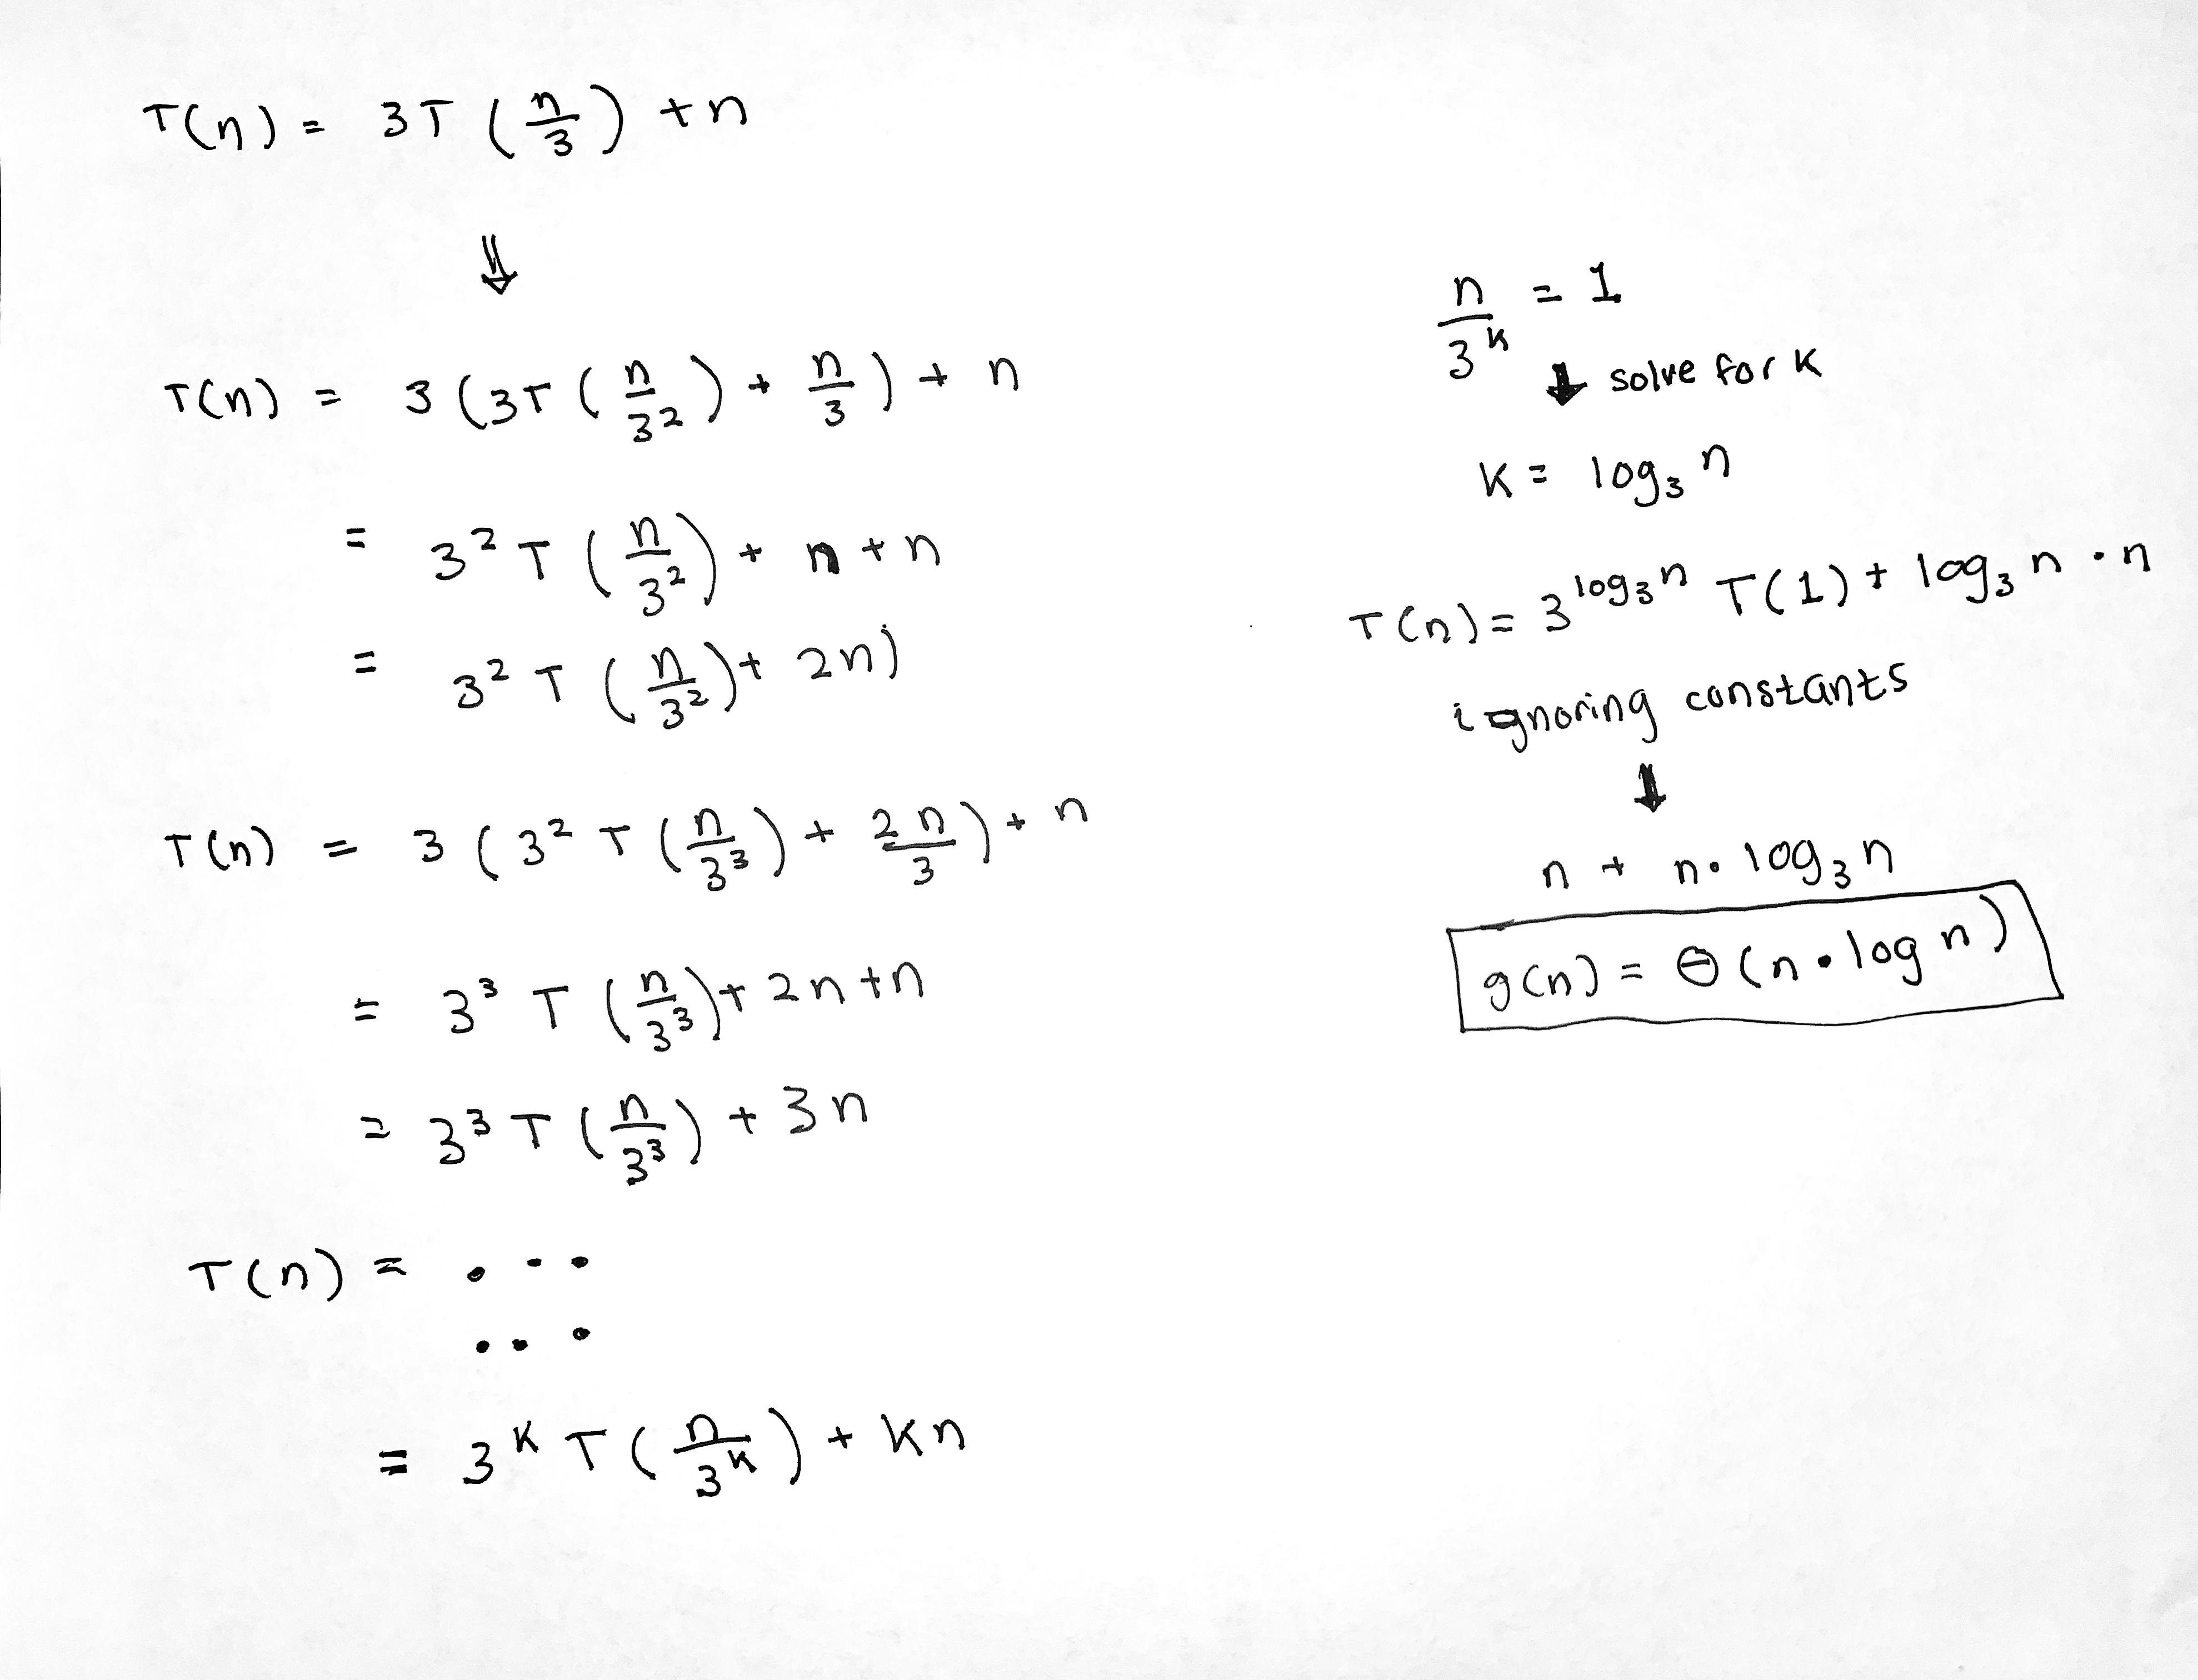
\includegraphics[scale=0.1]{solution4.jpg}
	    \\
	    \\
	    $T(n)= \Theta(n\cdot \log n)$
	}
	\item{\textit{(5 pts)
	Consider the following pseudo-code.}
	\begin{Verbatim}[numbers=left,xleftmargin=15mm, numbersep=10pt]
def fun(A[1,2,3....n]) {
    if A.length == 0:
        return 0
    count = 1
    for i=1 to n:
        for j=1 to n:
            count++
    return 1 + fun(A[1,2,3.....n-2])
}	        
	    \end{Verbatim}
	    \textit{Find a recurrence for the worst-case runtime complexity of this algorithm. Then solve
your recurrence and get a tight bound on the worst-case runtime complexity}.
	}
    \makenonemptybox{4.5in}{
    Evaluating time complexity of each line we get:\\
    $T(n)= c\cdot\mathcal{O}(1)+\mathcal{O}(n^2)+T(n-2)$\\
    disregarding the constants we get:\\
    $T(n)= \mathcal{O}(n^2)+ T(n-2)$\\
    solving the recurrence relation we get $T(n)= \mathcal{O}(n^3)$\\
    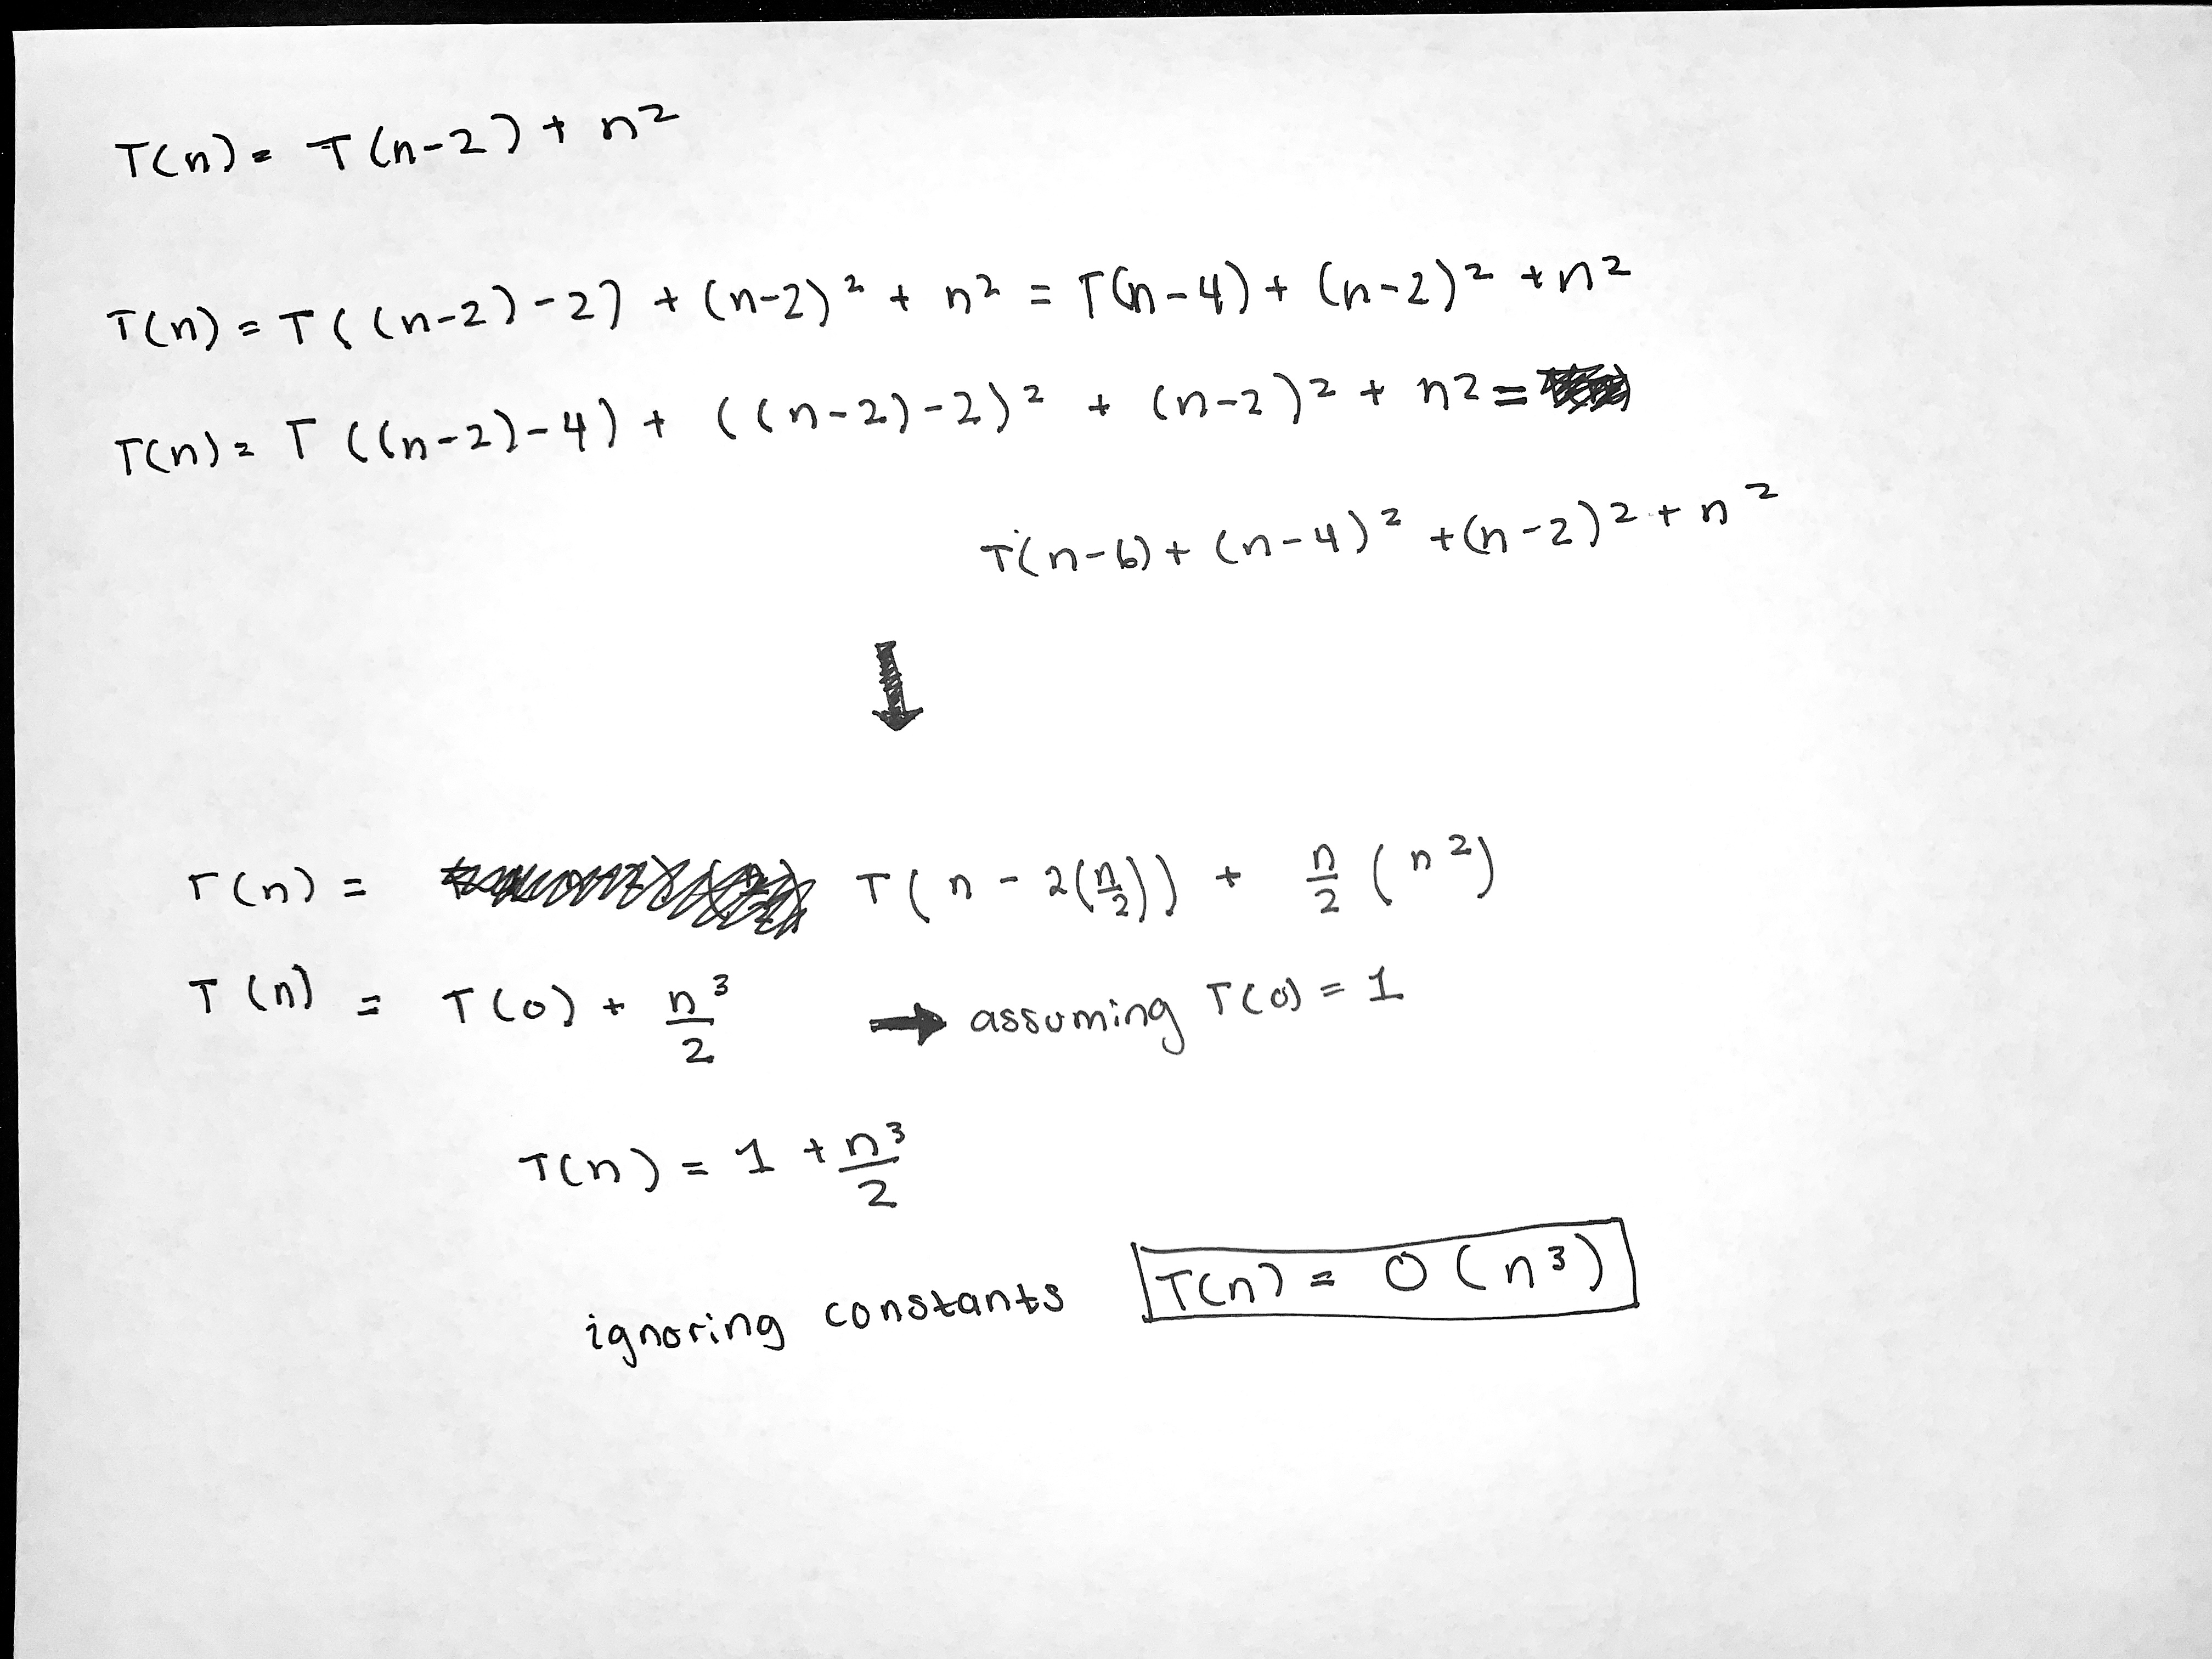
\includegraphics[scale=0.08]{solution5.jpg}
	}
	

\pagebreak
    
    \item{\itshape \textbf{Extra Credit (5\% of total homework grade)}
    For this extra credit question, please refer the leetcode link provided below or click \href{https://leetcode.com/problems/maximum-subarray/}{here}. Multiple solutions exist to this question ranging from brute force to the most optimal one. Points will be provided based on Time and Space Complexities relative to that of the most optimal solution.

    Please provide your solution with proper comments which carries points as well.}
    
   \url{https://leetcode.com/problems/maximum-subarray/}

    % Paste your code in the verbatim tag below
\begin{verbatim}
Replace this text with your source code inside of the .tex document
\end{verbatim}
	
\end{enumerate}


\end{document}


